\section*{PROPOSED HYBRID METHOD}\label{proposed-hybrid-method}

A hybrid method is proposed in this paper, where wave damping $B_W$
(including the speed dependent wave damping) obtained implicitly with
FNPF is used together with the viscous damping contributions from
Ikeda's method. The viscous damping is added to the FNPF simulations by
injecting the viscous parts of the linear and quadratic damping
coefficients (obtained with Ikeda's method) to the equation of motion.

Ikeda's method divides roll damping into five damping components so that
the total damping can be calculated as \citep{7505983/937PN5DT},

\begin{equation}
B = B_F + B_E + B_L + B_W + B_{BK}
\end{equation}

Where $B_F$ is the skin friction component, $B_E$ is the eddy
generation component, $B_L$ is hull lift component, $B_W$ is roll
wave generation component and $B_{BK}$ is the bilge keel component.

Ikeda's method propose semi empirical formulas for the viscous damping
components: $B_F$, $B_E$, $B_{BK}$ and $B_L$ so that viscous
damping can be obtained from,

\begin{equation}
\label{eq:viscous damping}
B_{visc} = B_F + B_E + B_L
\end{equation}

In order to reduce the number of uncertain parameters, the bilge keel
damping $B_{BK}$ has been exluded above, thereby assuming that the
ship does not have any bilge keels.

Many of the papers describing the Ikeda's method are translations from
original manuscripts written in Japanese. Summaries of this method
\citep{7505983/FB64RGPF}, \citep{7505983/KAKIM2E2} and
\citep{7505983/UGK6YEVD} have been used together with the original papers
to understand how the method should be implemented.
\citep{7505983/UGK6YEVD}

    

    
    \begin{figure}[H]
        \begin{center}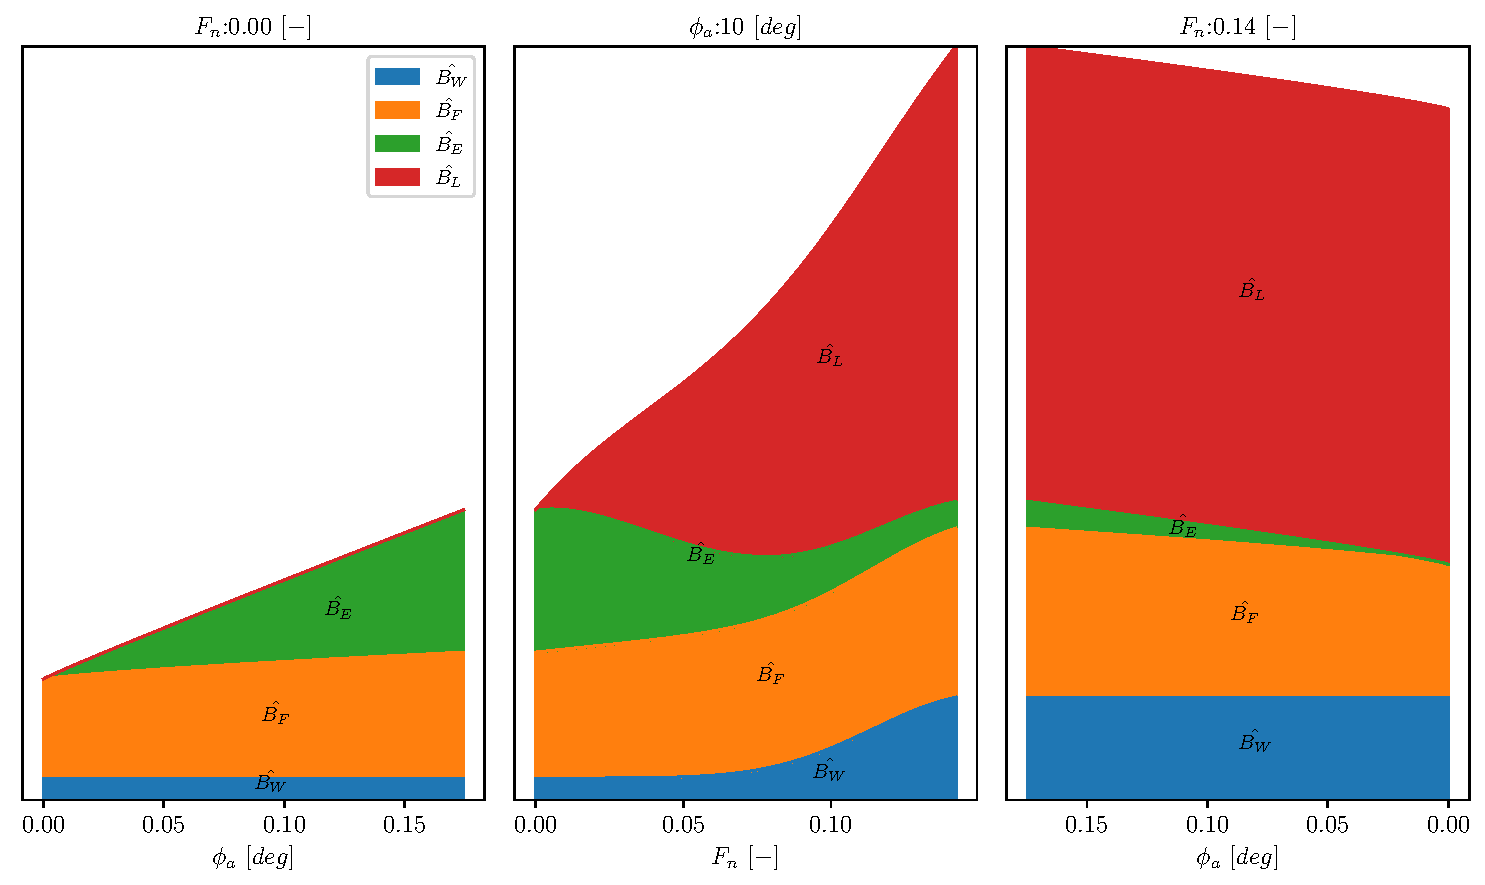
\includegraphics[width = 0.5\textwidth]{figures/ikeda_generic.pdf}\end{center}
        \vspace{-1cm}
        \caption{Example of roll damping predicted with Ikeda's method}
        \label{fig:ikeda_generic}
    \end{figure}
    
    When the damping predicted with Ikeda's method was compared with
corresponding model test it was found that the results were in poor
agreement for the zero speed case but quite good results at speed. This
was pointing towards the eddy damping being incorrect in the current
implementation of Ikeda's method. A thorough investigation of the eddy
damping prediction was therefore conducted which is described in the
next section.

    \subsection*{Eddy damping}\label{eddy-damping}

The eddy damping is due to eddies generated around the ship hull during
the roll motion. Strong eddies occures at sharp edges in the geometry.
Fig.\ref{fig:eddy_sigma} is an illustration of how the eddy
damping changes with bilge radius to beam ratio as predicted with the
current implementation of the method. It seems that the damping
approaches zero very fast as the bilge radius increase. So having just a
small rounding of the bilge, compared to a square section, will have a
great impact on the eddy roll damping.

    

    \begin{figure}[H]
        \begin{center}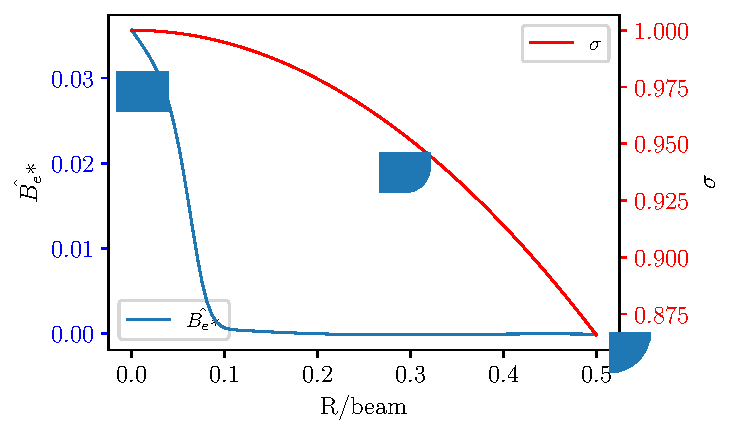
\includegraphics[width = 0.5\textwidth]{figures/eddy_sigma.pdf}\end{center}
        \vspace{-1cm}
        \caption{Eddy damping for various bilge radius}
        \label{fig:eddy_sigma}
    \end{figure}
    
    Ikeda made experiements on a number of two-dimensional cylinders with
various sections \citep{7505983/4AFVVGNT}. Ikeda found that the eddy
damping per unit length of these sections can be expressed as: 
 
            
    
    \begin{equation}
B'_{E0} = \frac{4 C_{r} T_{s}^{4} \omega \phi_{a} \rho}{3 \pi}
\label{eq:eddy_section}
\end{equation}

    

    The total eddy damping can be obtained as an integral over the sections
along the ship hull:
 
            
    
    \begin{equation}
B_{E0} = \int\limits_{AP}^{FP} B'_{E0}\, dx_{s}
\label{eq:eddy_integration}
\end{equation}

    

    It can be seen from the section damping (eq.
\ref{eq:eddy_section}) above that the eddy damping increases
linearly with both roll amplitude and frequency, and that it will go to
zero for small amplitudes and frequencies, which means that it is only
included in the quadratic damping term ($B_2$). Ikeda expressed the
$C_r$ coefficient to be entirely depending on the hull form. Ikeda
developed a regression formula for $C_r$ based on his experiments,
which is used in the prediction method. The authors of this paper have
tried to implement this method according to the description in the
original paper \citep{7505983/4AFVVGNT} but have failed to reproduce the
results from Ikeda's experiments exactly. Other resources such as
\citep{7505983/FB64RGPF} and \citep{7505983/KAKIM2E2} have also been used
without success.

Instead, a new regression for $C_r$ was made on the experimental
results from \citep{7505983/4AFVVGNT}. The experimental results were
collected by the authors using manual digitalization
\citep{7505983/RXYIE6UW}.

    The nondimensional damping is expressed in \citep{7505983/4AFVVGNT} using
an asterisk, or star symbol (*). The reason seems to be that Ikeda
wanted to signal that this damping only has the quadratic part of the
damping. This stared damping is defined as:
 
            
    
    \begin{equation}
\hat{B}_{E0} = \frac{8 \hat{B^*}_{E}}{3 \pi}
\label{eq:B_E_star_hat}
\end{equation}

    

    $\hat{B_E^*}$ and $(B_W+B_F)^*$ are the experimental values taken
from \citep{7505983/4AFVVGNT}. Which add up to the total damping:

    $\hat{B^*} = \hat{B^*_E} + (B_W+B_F)^*$

    And the $C_r$ was calculated from the experiments as:
 
            
    
    \begin{equation}
C_{r} = \frac{3 \pi B_{s} T_{s} \hat{B}_{E0} beam^{2} \sigma}{4 T^{4} \hat{\omega} \phi_{a}}
\label{eq:C_r_2}
\end{equation}

    

    Instead of trying to invent a complicated mathematical expression for
the $C_r$ regression a simple decision tree model, based on the Lewis
section coefficients, was instead fitted to the $C_r$ data from
Ikeda's experiments. The fitted decision tree is illustrated in
Fig.\ref{fig:decision_tree}.

    

    \begin{figure}[H]
        \begin{center}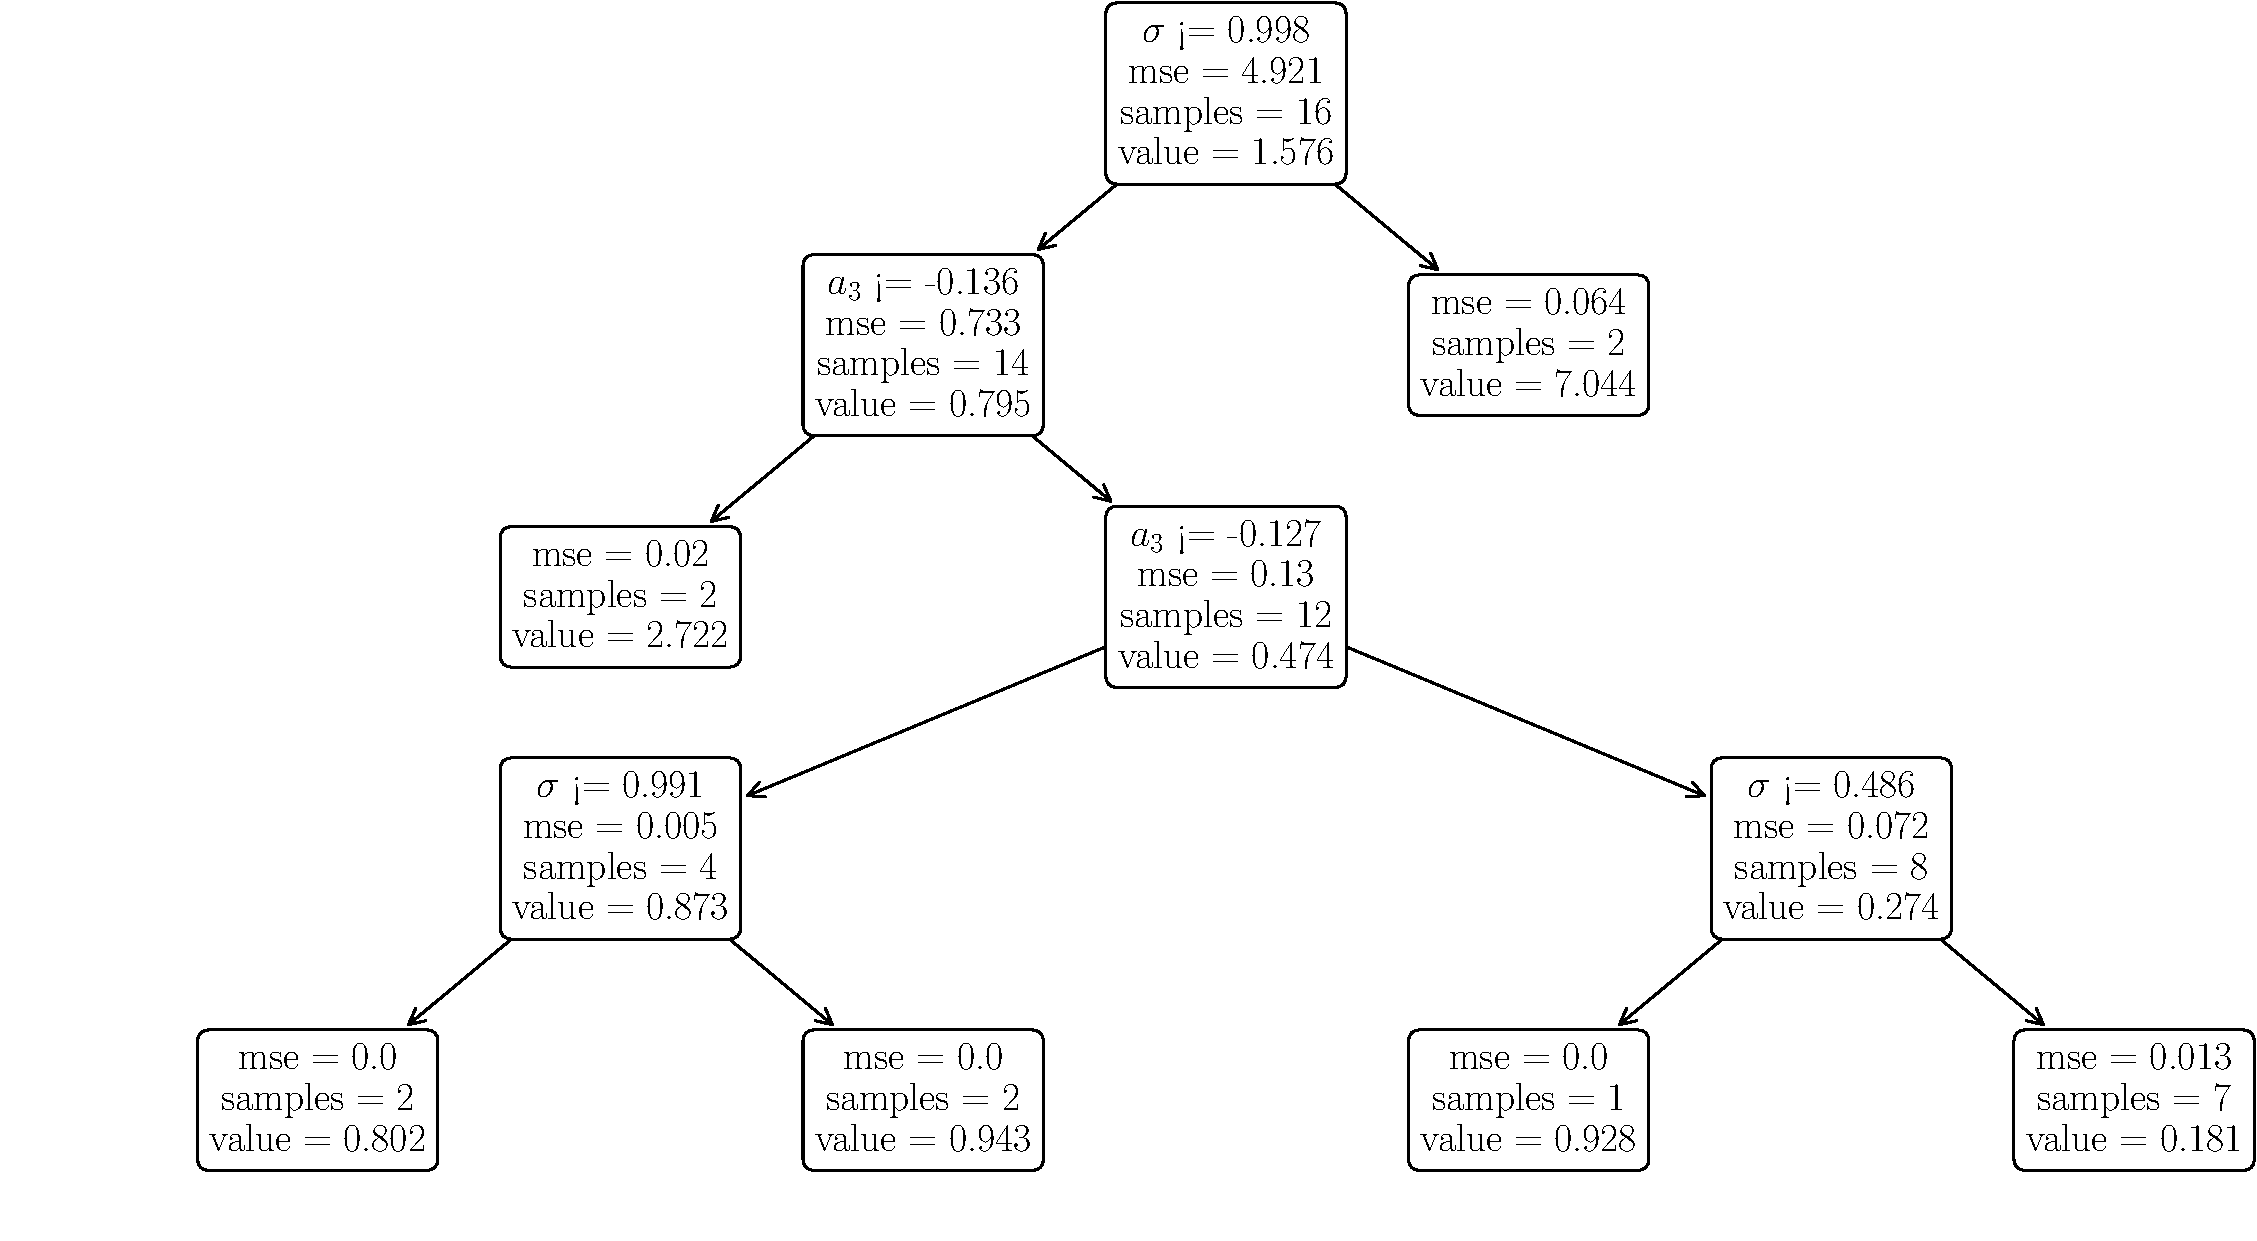
\includegraphics[width = 0.5\textwidth]{figures/decision_tree.pdf}\end{center}
        \vspace{-1cm}
        \caption{Decision tree}
        \label{fig:decision_tree}
    \end{figure}
    
    Even thoug this tree is very simple it has very good accuracy in
reproducing the results from Ikedas experiments ($r^2=0.996)$.

    \subsection*{FNPF method}\label{fnpf-method}

\label{fnpf-method} Wave damping was obtained using PIT on roll decay
simulation using the fully nonlinear potential flow method. This method
is characterized by the application of the complete dynamic and
kinematic free surface boundary conditions on the instantaneous free
surface as well as the body-exact approach where the instantaneous
wetted body surface is considered in the boundary value problem for the
velocity potential, i.e. no linearizations are made to the governing
equations of the potential flow problem.

The method used in this study employs a boundary element method (BEM)
\citep{7505983/FD4N3DW2} to solve the boundary value problem for the
velocity potential.

The free surface boundary conditions and the motions of the floating
body introduce time dependency to the boundary value problem. The BEM is
coupled with the mixed Eulerian-Lagrangian method (MEL)
\citep{7505983/ZKB494GT} which is used for the evolution of free surface.
A fourth-order Adams-Bashforth-Moulton time integral scheme is then used
to evolve free surface and the rigid-body body motions in time.

The benefit with the FNPF method is the lack of linearizations to the
free surface potential flow where all interactions between the
undisturbed incident flow and surface piercing body is captured
implicitly in the total velocity potential, including inviscid (wave)
damping due to radiation and diffraction. The downside is the larger
computational cost compared to many other potential flow based methods
due to the fact that a boundary value problem for the velocity potential
must be solved at least once every time step, depending on the specifics
of the time integral scheme. However, FNPF methods are still typically
less computationally demanding than for example URANS methods, making
them attractive choices for seakeeping problems.

    